\documentclass[12pt,twoside]{article}
\usepackage{jmlda}
\usepackage{url}
\usepackage{hyperref}
\usepackage{graphicx}

\makeatletter
\bibliographystyle{unsrt}
\renewcommand{\@biblabel}[1]{#1.}
\makeatother
\pgfplotsset{compat=1.18} 
%\NOREVIEWERNOTES
\title
    [Классификация фазовой траектории] 
    % Краткое название; не нужно, если полное название влезает в~колонтитул
    {Классификация квазипериодических временных сигналов с помощью сферических гармоник}
\author
    {Тихонов~Д.\,М., Стрижов~В.\,В.} % основной список авторов, выводимый в оглавление
    %\thanks
    %{Работа выполнена при финансовой поддержке РФФИ, проект \No\,00-00-00000.}
%\email
   % {author@site.ru}
% \organization
%   {$^1$Организация; $^2$Организация}
%\thanks
%	{ }
\abstract
{\textbf{Аннотация}: Решается задача построения модели аппроксимации и классификации квазипериодических сигналов.
Требуется наименьшая структурная сложность.
Структурная сложность~---~это число настраиваемых параметров модели.
Для перехода в фазовое пространство временной ряд векторизуется с помощью метода задержек.
Для понижения сложности модели в фазовом пространстве выбирается подпространство.
Фазовая траектория в полученном подпространстве аппроксимируется линейной комбинацией сферических гармоник.
Полученные коэффициенты используются в качестве признакового описания.
Вычислительный эксперимент проведен на измерениях акселерометра мобильного устройства с тремя классами движений человека.

\bigskip
\textbf{Ключевые слова}: \emph {временные ряды, апрроксимация, классификация, фазовое пространство, сферические гармоники}.}

\newcommand{\nsymbol}[2]{\medskip\hangindent=\parindent\hangafter=1\noindent $#1$ --- #2\par}
\newcommand{\nsymbolp}[3]{\nsymbol{#1}{#2 \dotfill\pageref{#3}}}

\newcommand{\hookuparrow}{\mathrel{\rotatebox[origin=t]{270}{$\hookleftarrow$}}}
\newcommand{\hookdownarrow}{\mathrel{\rotatebox[origin=t]{90}{$\hookleftarrow$}}}
\begin{document}
\maketitle

\section{Введение}
Работа посвящена классификации квазипериодических временных рядов.
Примерами таких рядов являются показатели акселерометра и гироскопа во время повторяющейся физической активности, электрокардиограмма.

Классическим подходом является использование метода ближайших соседей в сочетании с различными функциями расстояния~\cite{Bagnall_2017}, либо ансамбль различных типов дискриминативных моделей на одном или нескольких пространствах признаков~\cite{Hills_2014, Bostrom2017, Kate_2015}.
Эти походы имеют общее свойство: этап преобразования данных, на котором временные ряды преобразуются в новое пространство признаков,например, с помощью шейплет преобразований ~\cite{ Hills_2014, Bostrom2017} или функции DTW~\cite{Kate_2015}.
Другой широкий класс подходов к решению~---~это использование различных нейронных сетей на исходных временных рядах~\cite{WANG_2019}, например, с помощью операции свертки.
Методы объединяющие подход порождения признаков и прямое использования временных рядов основаны на методе задержек и классификации полученных векторных представлений~\cite{Frank_2010}.
Последний является ближайшим подходом к решению, описанному в данной работе и альтернативным подходом для сравнения.

В этой работе предлагается модель классификации временных рядов, основанный на модели аппроксимации сферическими гармониками на поверхности сферы. 
Для этого производится переход в пространство фазовых траекторий или траекторное пространстве.
Переход осуществляется методом задержек~\cite{LAI19961}.
Метод задержек используется при анализе нестационарных временных рядов.
Например, в методе сингулярного спектрального анализа~\cite{Golyandina2002} разложения на компоненты и прогноз основаны на траекторной матрице.
Она позволяет перейти от скалярного временного ряда к многомерному представлению.
Метод задержек так же получили широкое распространение в анализе нелинейных динамических систем~\cite{Takens1981, LAI19961}.

Избыточная размерность траекторного пространства ~\cite{Golyandina2002, Motrenko2015,Usmanova2020} приводит к неустойчивости исследуемых моделей и избыточно сложному описанию временного ряда.
Для понижения размерности фазового пространства предлагается использовать  метод главных компонент~\cite{Ezukwoke2019, Scholkopf1998}.

\begin{figure}[h]
\centering
%   \subfloat[$s(t) = 2cos(2\pi\nu_1t + \varphi_1) + cos(2\pi\nu_2t + \varphi_2) + \varepsilon$]
  {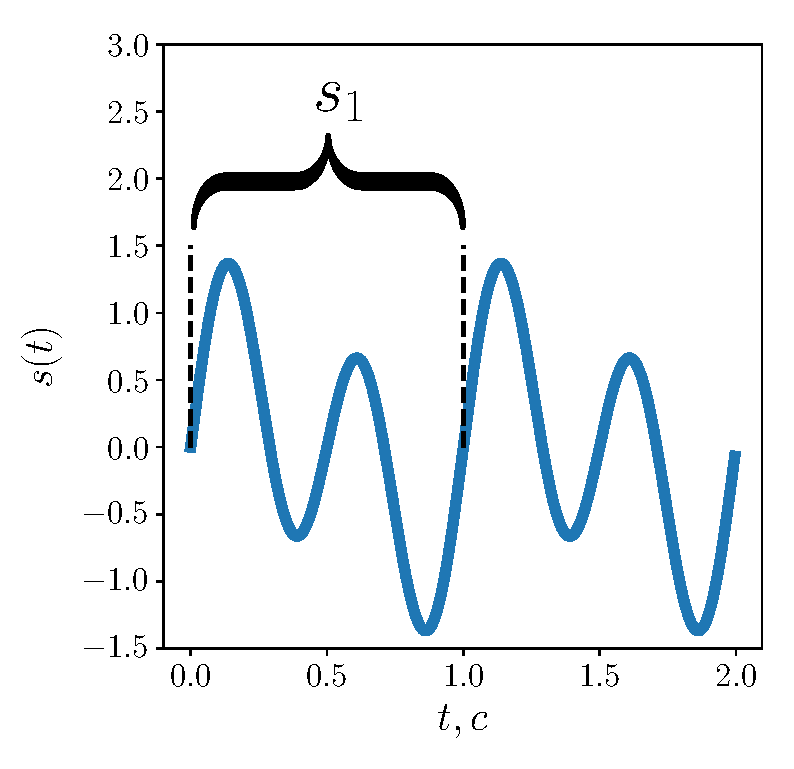
\includegraphics[width=0.25\textwidth]{figs/synthetic_example.eps}}
%   \subfloat[Фазовая траектория (PCA)]
  {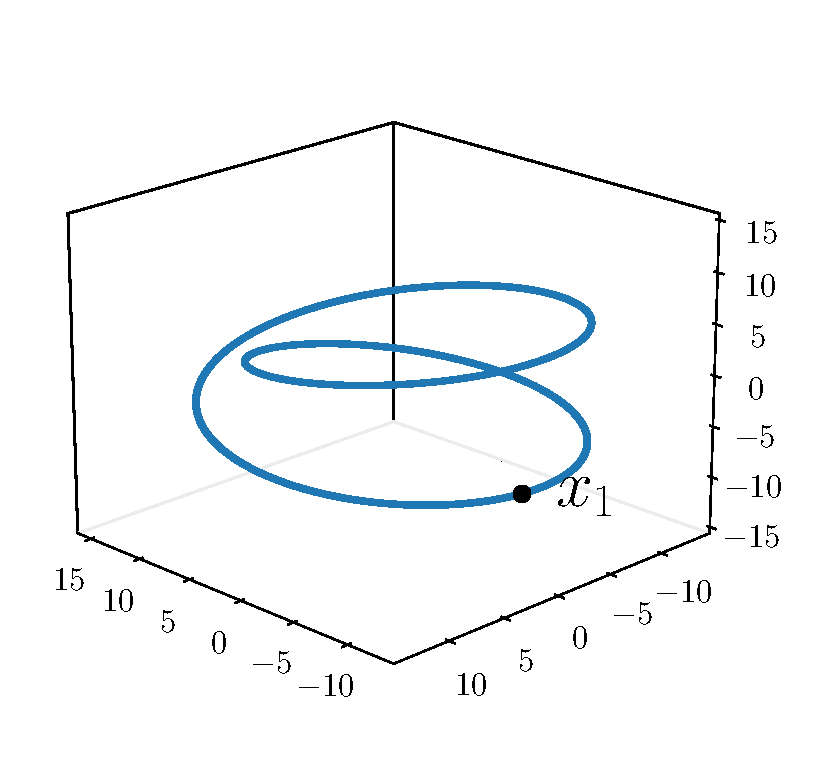
\includegraphics[width=0.3\textwidth]{figs/synthetic_trajectory.eps}}\\
\caption{Слева: сегмент временного ряда, справа: фазовая траектория.}
\label{fg:initial_traj}
\end{figure}

В выбранном фазовом подпространстве малой размерности фазовая траектория проецируется на $p$-мерную единичную сферу.
Полученную на поверхности сферы функцию предлагается аппроксимировать линейной комбинацией сферических гармоник.
Полученные коэффициенты в дальнейшем используются как признаковое описание в задаче классификации.

На Рис.~\ref{fg:initial_traj} показан сегмент синтетического временного ряда и его фазовая траектория в пространство размерности три.
Фазовая траектория получена с помощью метода задержек и метода главных компонент над матрице задержек.

%%%%%%%%%%%%%%%%%%%%%%%%%%%%%%%%%%%%%%%%%%%%%%%%%%%%%%%%%%%%%%%%%%%%%%%%%%%%%
\section{Постановка задачи классификации сферическими гармониками}

Пусть заданы $\mathbf{S}$ --- множество временных рядов, $\mathbf{Z}$ --- множество номеров классов.
Требуется по конечной выборке $\mathbf{S}^{b} = \{(\mathbf{s}_1, y_1),\dots,(\mathbf{s}_{b}, y_{b}) \}$ , где  $\mathbf{s}=[s_1,...,s_N]$ --- временной ряд, $b$ --- число объектов в выборке, построить отображение
\begin{equation}
y*:\mathbf{S} \xrightarrow{} \mathbf{Z}.
\label{eq:y*}
\end{equation}

По имеющемуся временному ряду $\mathbf{s}$ строится траекторная матрица

\begin{equation*}
    \mathbf{H}_{s}^{n} = 
    \begin{bmatrix} 
    	s_{1} & s_{2} & \ldots &s_{n-1} &s_{n}\\
    	s_{2} & s_{3} & \ldots &s_{n} &s_{n+1}\\
    	\vdots& \vdots & \ddots & \vdots & \vdots\\
    	s_{N-n+1} & s_{N-n+2} &\ldots&s_{N-1} &s_{N}\\
    \end{bmatrix} = 
	\begin{bmatrix} 
      	\mathbf{s}_{1}\\
      	\mathbf{s}_{2}\\
      	\vdots\\
      	\mathbf{s}_{m}\\
   \end{bmatrix},
   \quad
   m = N-n+1,
\label{eq:hankel_matrix}
\end{equation*}
где $N$~---~длина временного ряда, $n$~---~ширина окна, не меньшая, чем предполагаемый период,  $\mathbf{s}_t=[s_{t},s_{t+1},\ldots,s_{t+n-1}] \in \mathbb{H}_{s} \subseteq \mathbb{R}^{n}$ --- векторы, образующие фазовую траекторию ряда $\mathbf{s}$.

Размерность траекторного пространства $\mathbb{H}_{s}^{n}$ избыточна.
Предлагается снижать размерность $\mathbb{H}_{s}^{n} \xrightarrow{} \mathbb{H}_{x}^{p}$ с помощью метода главных компонент при $p \ll n $:
\begin{equation}
\mathbf{H}_{x}^{p} = \mathbf{H}_{s}^{n}\mathbf{U} =
\begin{bmatrix} 
  	\mathbf{x}_{1}\\
  	\mathbf{x}_{2}\\
  	\vdots\\
  	\mathbf{x}_{m}\\
\end{bmatrix},
\quad
\mathbf{x}_{t} \in \mathbb{R}^{p},
\quad
t \in [1,m]
\label{eq:PCA}
\end{equation}
где $\mathbf{U}$ --- матрица преобразования алгоритма метода главных компонент с количеством компонент равным $p$, соответствующим наибольшим собственным значениям.

В полученном подпространстве фазовая траектория переводится из декартовых в сферические координаты $\mathbb{H}_{x}^{p} \xrightarrow{} \mathbb{S}_{r}^{p}$:
\[
    \phi: \mathbf{x} \xrightarrow{} \mathbf{r} = [r,\alpha_{p-1},\dots,\alpha_1],
    \quad
    \mathbf{a} = [\alpha_{p-1},\dots,\alpha_1],
    \quad
    \mathbf{S}_{r}^{p} = \phi(\mathbf{H}_{x}^{p}).
\]

По полученным представлениям точек в пространстве $\mathbb{S}^{p}$ строится модель фазовой траектории как линейная комбинация сферических гармоник.

Предлагается представить $y*$~(\ref{eq:y*}) как суперпозицию отображений
\begin{equation*}
t \mapsto \mathbf{s} \mapsto \mathbb{H}_{s}^{n} \xrightarrow{} \mathbb{H}_{x}^{p} \xrightarrow{} \mathbb{S}_r^{p} \xrightarrow{} \mathbb{W}^{p-1} \xrightarrow{} \mathbf{Z},
\label{tikhonov_eq_pipeline}
\end{equation*}
где $\mathbb{W}^{p-1}$~---~пространство весов модели аппроксимации, $\mathbb{H}_{s}^{n}$~---~фазовое пространство, полученное методом задержек, $\mathbb{H}_{x}^{p}$~---~фазовое подпространство в декартовых координатах, $\mathbb{S}_{r}^{p}$~---~фазовое подпространство в сферических координатах.
%%%%%%%%%%%%%%%%%%%%%%%%%%%%%%%%%%%%%%%%%%%%%%%%%%%%%%%%%%%%%%%%%%%%%%%%%%%%%
\section{Модель фазовой траектории}
В полученном подпространстве $\mathbb{S}^{p}$ строится модель фазовой траектории
\begin{equation}
    f_{\text{sp}}: \mathbb{R}^{|\mathbf{w}_{\text{sp}}|} \times \mathbb{S}_{r}^{p}
    \xrightarrow{}
    \mathbb{R}.
\label{eq:f_sp}
\end{equation}

Нормированные значения функции $f_{\text{sp}}$ интерпретируются как вероятность принадлежности точки фазового пространства $\mathbb{S}$ к фазовой траектории $\mathbf{S}$ временного ряда $\mathbf{s}$

\begin{equation}
	\pi(\mathbf{a}) \approx
	f_{\text{sh}}(\mathbf{w}_{\text{sp}},\mathbf{a}) =
	\sum_{l_{p-1} = 0}^{N_{\text{approx}}}
	\sum_{l_{p-2} = 0}^{l_{p-1}}
	\dots
	\sum_{l_1 = -l_2}^{l_2}
	w_{l_{p-1},...,l_1} Y_{l_{p-1},...,l_1}(\mathbf{a}),
\label{eq:f_sh}
\end{equation}
где $\pi(\mathbf{a})$~---~ функция проекций, определенная ниже, $l_{p-1},...,l_1$~---~индексы, определяющие сферические гармоники и удовлетворяющие условию $l_{p-1} \geq l_{p-2} \dots l_2 \geq|l_1|$, $N_{\text{approx}}$~---~максимальное значения старшего индекса, $Y_{l_{p-1},...,l_1}(\mathbf{a})$~---~вещественные сферические гармоники, определенные ниже, $w_{l_{p-1},...,l_1}$~---~ весовые коэффициенты $w_{l_{p-1},...,l_1} \in \mathbb{W}^{p-1}$.
$N_{\text{approx}}$ связан с точностью модели, чем больше значение, тем точнее аппроксимация и больше переобучение. 
 
В качестве базисных функций на поверхности $(p-1)$-мерной сферы используются сферические гармоники:

\begin{equation}
	\mathcal{Y}_{l_{p-1},...,l_1}(\alpha_{p-1},\dots,\alpha_1) = 
	\left[
	    \prod\limits_{k = 2}^{p-1}
	    {\overline{\text{P}}}_{l_k}^{l_{k-1}}(\alpha_k)
	\right]
	    \frac{1}{\sqrt{2\pi}}
	    \exp{(\pm i |l_1| \alpha_1)},
\label{eq:YlN}
\end{equation}

За функцию ${\overline{\text{P}}}_{l_k}^{l_{k-1}}(\alpha_k)$ обозначается  
\[
{\overline{\text{P}}}_{l_k}^{l_{k-1}}(\alpha) =
   c^{l_{k-1}}_{l_k} \cdot (\sin \alpha)^{\frac{-(k-2)}{2}}
   \text{P}^{-(l_{k-1}+\frac{(k-2)}{2})}_{l_k+\frac{(k-2)}{2}}(\cos \alpha),
   \quad
   c^{l_{k-1}}_{l_k} = 
        \sqrt{
	        \frac{2l_{k-1}+k-1}{2}
	        \frac{(l_k+l_{k-1}+k-2)!}{(l_k-l_{k-1})!}
	    }
\]
\noindentгде $\text{P}_{\mu}^{-\eta}(x)$ --- полиномы Лежандра, $c^{l_{k-1}}_{l_k}$ --- нормировочный коэффициент.
Подробнее о выводе формул и введенных обозначениях в 

Сферические гармониками определены в комплексном пространстве.
В исследуемом случае нет необходимости в реальной и комплексной части одновременно.
Используются только вещественные сферические гармоники.
Это упрощает реализацию и сохраняет свойства ортонормированности.
Так вещественные сферические гармоники представимы в следующем виде

\begin{equation}
	Y_{l_{p-1},...,l_1}(\alpha_{p-1},\dots,\alpha_1) = \begin{cases}
	\text{Re}(\mathcal{Y}_{l_{p-1},...,l_1}(\alpha_{p-1},\dots,\alpha_1)), & \mbox{если } l_1 \geq 0\\
    \text{Im}(\mathcal{Y}_{l_{p-1},...,l_1}(\alpha_{p-1},\dots,\alpha_1)), & \mbox{иначе}.
    \end{cases}
\label{eq:RTY}
\end{equation}

Для расчета $w_{l_{p-1},...,l_1}$ весовых коэффициентов в~(\ref{eq:f_sh}) необходимо определить проекцию фазовой траектории $\pi(\mathbf{a})$ на поверхности сферы $\mathbb{S}^{p-1}$.
Для этого поверхность сферы разбивается на области, как показано слева на Рис.~\ref{fg:sp_mesh}.

\begin{figure}[h]
\centering
  {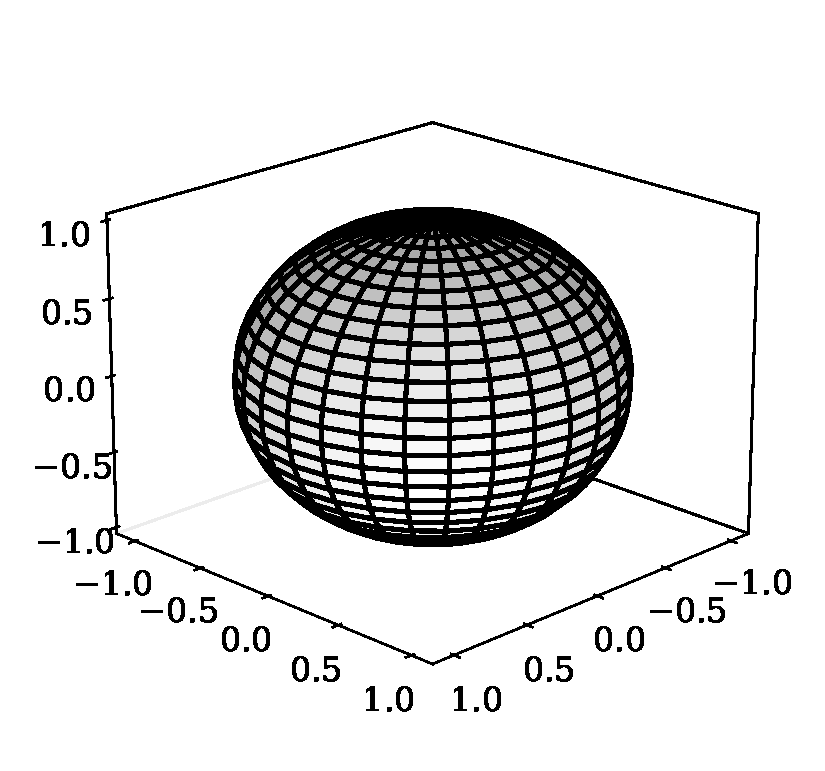
\includegraphics[width=0.3\textwidth]{figs/sphere_grid.eps}}
  {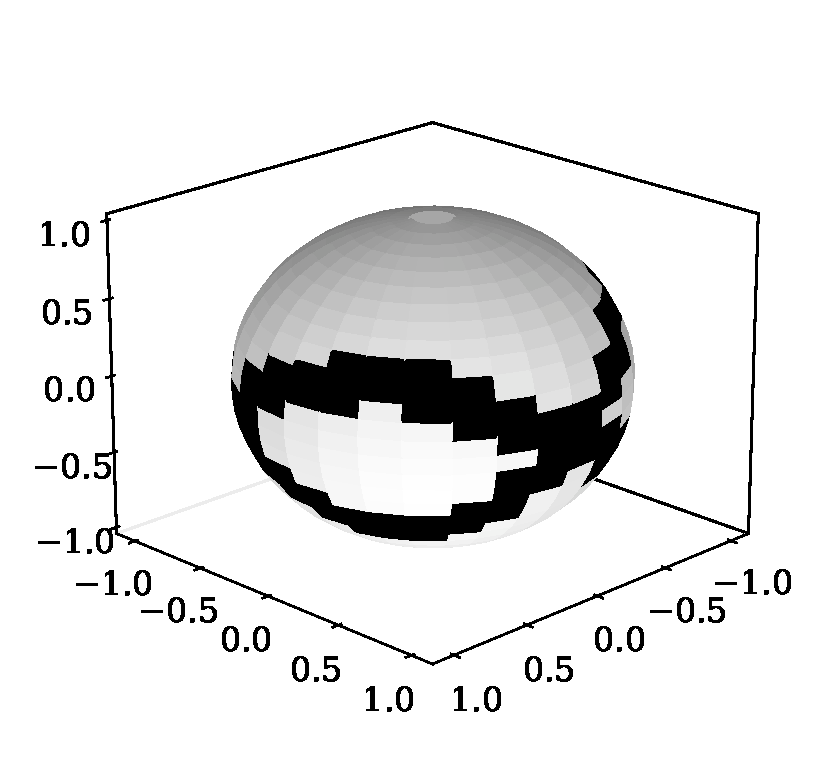
\includegraphics[width=0.3\textwidth]{figs/pi_walk.eps}}\\
\caption{Слева: области на сфере, справа: полученная проекция.}
\label{fg:sp_mesh}
\end{figure}

По полученному разбиению $\mathbb{A}^{p-1}$ на сфере и по точкам фазовой траектории строится функция проекции $\pi(\mathbf{a}), \mathbf{a} \in \mathbb{A}^{p-1}$

\begin{equation}
    \pi(\mathbf{a}) =
    \begin{cases}
	1, & \mbox{если } \mathbf{a} \in \mathbb{A}^{p-1} \cap \mathbf{S}_{z}^{p},\\
    0, & \mbox{если } \mathbf{a} \in \mathbb{A}^{p-1} \setminus \mathbf{S}_{z}^{p}.
    \end{cases}
\label{eq:f_real}
\end{equation}
Пример проекции справа на Рис.~\ref{fg:sp_mesh}.

Составляется система относительно весовых коэффициентов $w_{l_{p-1},...,l_1}$ 

\begin{equation}
\begin{pmatrix} 
	{Y}_{l_{p-1},...,l_1}({\mathbf{a}}_1) & \ldots & {Y}_{0,...,0}({\mathbf{a}}_1)\\
	\vdots& \ddots & \vdots\\
	{Y}_{l_{p-1},...,l_1}({\mathbf{a}}_d) & \ldots & {Y}_{0,...,0}({\mathbf{a}}_d)\\
\end{pmatrix}
\begin{pmatrix} 
	w_{l_{p-1},...,l_1}\\
	\vdots\\
	w_{0,...,0}\\
\end{pmatrix}
=
\begin{pmatrix} 
	\pi(\mathbf{a}_1)\\
	\vdots\\
	\pi(\mathbf{a}_d)\\
\end{pmatrix},
\label{eq:sp_app_matrix}
\end{equation}
\noindentгде $Y_{l_{p-1},...,l_1}({\mathbf{a}}_i)$ --- значение сферической гармоники в точке ${\mathbf{a}}_i$, $d$ --- количество точке в сетке на сфере Рис.~\ref{fg:sp_mesh}.
В более короткой записи:
\begin{equation}
\mathbf{{Y}}\mathbf{w}_{\text{sp}} = \mathbf{\Pi}.
\label{eq:sp_app_matrix_short}
\end{equation}

Эта постановка сводит решения к МНК, что ускоряет процедуру расчета весовых коэффициентов.
В силу экспоненциального роста числа сферических гармоник при повышении размерности фазового пространства, вводятся регуляризаторы

\begin{equation}
    \mathbf{\hat{w}}_{\text{sp}} = \argmin_{\mathbf{w}_{\text{sp}}}
    \|\mathbf{{Y}}\mathbf{w}_{\text{sp}} - \mathbf{\Pi}\|^2 + \lambda\|\mathbf{w}_{\text{sp}}\|^2.
\label{eq:arg_l2}
\end{equation}
Решение представимо аналитически:
\begin{equation}
    \mathbf{\hat{w}}_{\text{sp}} = (\lambda \mathbf{I} - \mathbf{{Y}}^{\mathsf{T}}\mathbf{{Y}})^{-1}\mathbf{{Y}}^{\mathsf{T}}\mathbf{\Pi}.
\label{eq:arg_l2_solution}
\end{equation}

%%%%%%%%%%%%%%%%%%%%%%%%%%%%%%%%%%%%%%%%%%%%%%%%%%%%%%%%%%%%%%%%%%%%%%%%%%%%%
\section{Модель классификации весовых коэффициентов}

\begin{figure}[H]
\centering
\subfloat[Классификации с совместной матрицей PCA для всех классов]
{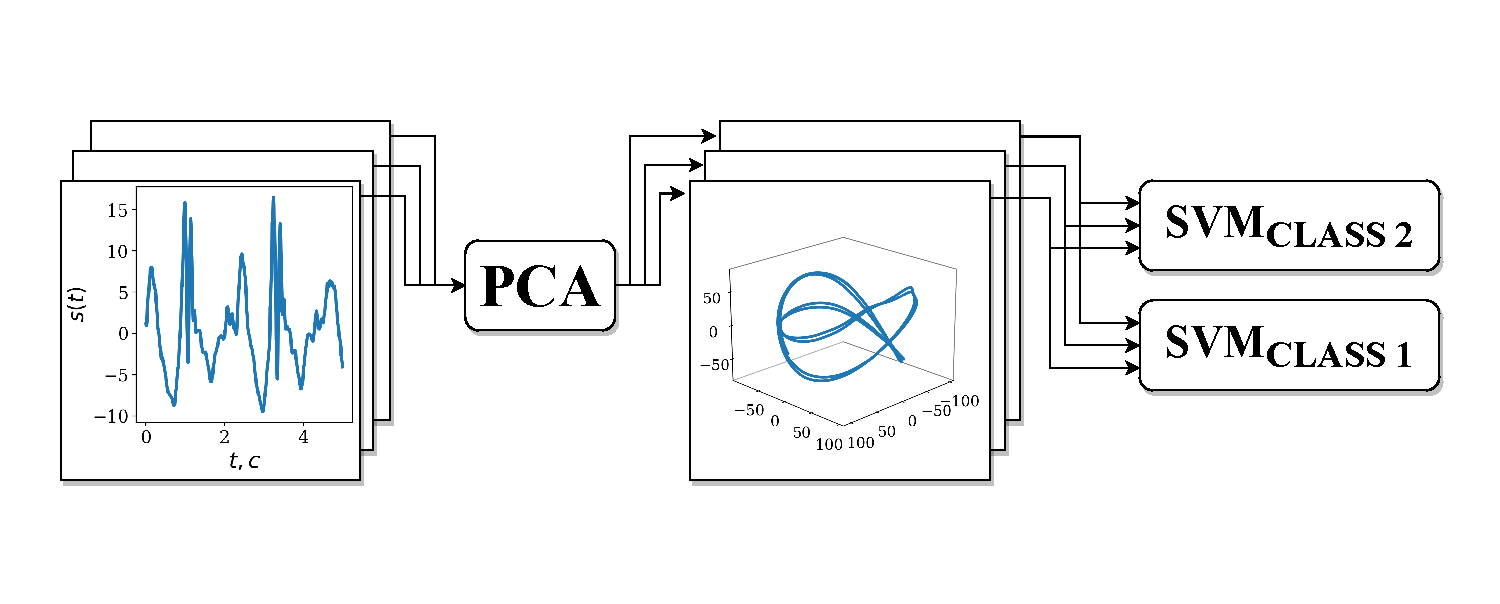
\includegraphics[scale=0.5]{./figs/PCA_SVM.pdf}}\\
\subfloat[Классификации с отдельной матрицей PCA для каждого класса]
{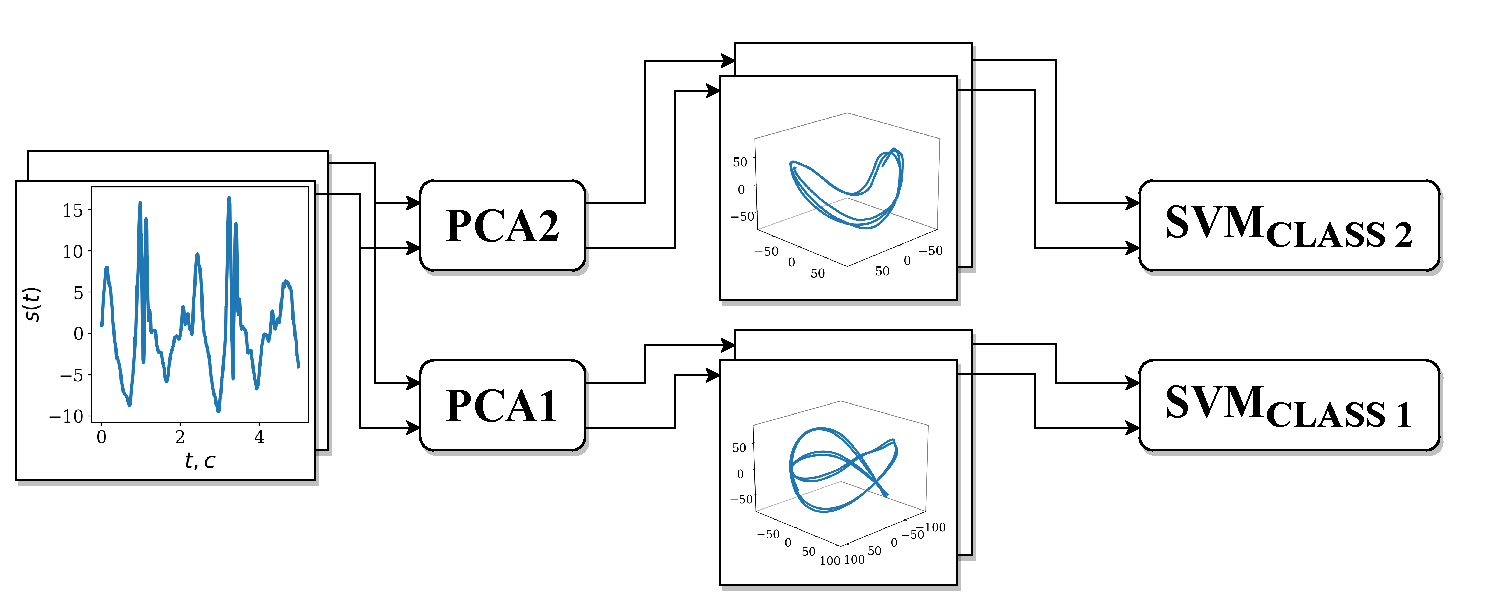
\includegraphics[scale=0.5]{./figs/TWO_UNIQUE_PCA_SVM.pdf}}\\
\subfloat[Предложенный метод классификации]
{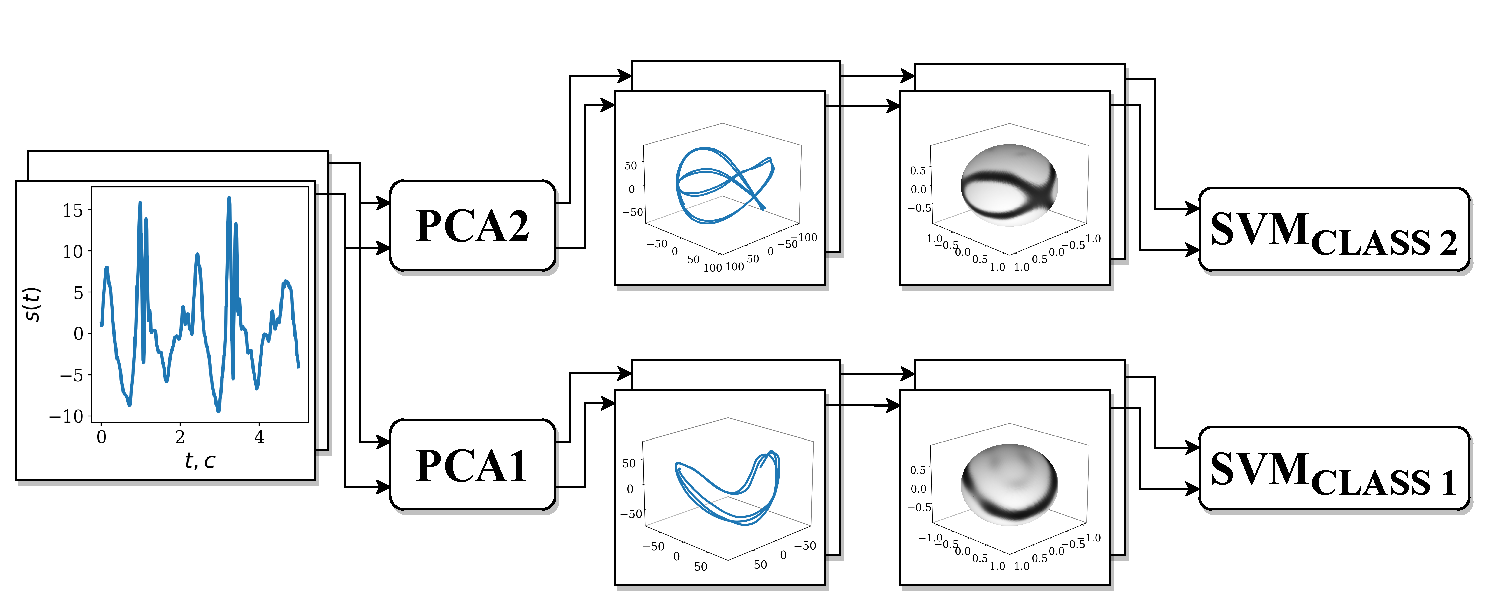
\includegraphics[scale=0.5]{./figs/PCA_HARM_SVM.pdf}}\\
\caption{Сравнение различных подходов к классификации фазовой траектории}
\label{fg:alternative_piplines}
\end{figure}

Полученные весовые коэффициенты~(\ref{eq:arg_l2_solution}) для каждого $\mathbf{s} \in \mathbf{S}^{b}$ используются в качестве признакового описания в задаче классификации. Для классификации используется метод опорных векторов с мягким зазором
 
\begin{equation}
    g(\mathbf{w}_{\text{sh}}) = \text{sign}(\mathbf{{w}}_{\text{svm}}^{\mathsf{T}}\,\mathbf{w}_{\text{sh}}).
\label{eq:svm}
\end{equation}

Весовые коэффициенты $\mathbf{{w}_{\text{svm}}}$~(\ref{eq:svm}) оптимизируются

\begin{equation}
\begin{cases}
    \frac{1}{2}\|\mathbf{{w}_{\text{svm}}}\|_2^2 + C\sum_{i=1}^{\hat{m}}\xi_i \xrightarrow{} \min_{{w}_{\text{svm}},\,\xi}\\
    y_i \cdot \mathbf{{w}}_{\text{svm}}^{\mathsf{T}}\mathbf{w}_{\text{sh },i} \geq 1 - \xi_i, \quad i = 1,\dots,b\\
    \xi_i \geq 0, \quad i = 1,\dots,b,\\
\end{cases}
\label{eq:svm_solutin}
\end{equation}
где $C$~---~параметр настройки метода, который позволяет регулировать отношение между максимизацией ширины разделяющей полосы и минимизацией суммарной ошибки, $\xi_i$~---~величина, характеризующая ошибку на объектах ${w}_{\text{svm }i}$. 

%%%%%%%%%%%%%%%%%%%%%%%%%%%%%%%%%%%%%%%%%%%%%%%%%%%%%%%%%%%%%%%%%%%%%%%%%%%%%
\section{Модель классификации точек фазовой траектории}
В качества альтернативы используется ближайшая по архитектуре модель описанная в~\cite{Frank_2010}. В этой работе классифицируются точки фазовой траектории $\mathbf{H}_{x}^{p}$ по стратегии One-Vs-Rest. Решается задача
\begin{equation}
    g(\mathbf{x}) = \text{sign}(\mathbf{{w}}_{\text{svm}}^{\mathsf{T}}\,\mathbf{x}),
    \quad
    \mathbf{x} \in \mathbf{H}_{x}^{p}.
\label{eq:alternative_svm}
\end{equation}

Сравниваются два варианта классификации.
В первом матрица преобразования метода главных компонент~(\ref{eq:PCA}) строится для объединения всех фазовых траекторий полученных методом задержек и далее классифицируется для каждого класса отдельным методом опорных векторов как показано на Рис.~\ref{fg:alternative_piplines}а.
Во втором варианте матрица преобразования метода главных компонент строится для каждого класса отдельно и далее классифицируется аналогично первому варианту как показано на Рис.~\ref{fg:alternative_piplines}б.

% \begin{figure}[h]
%     \centering
%     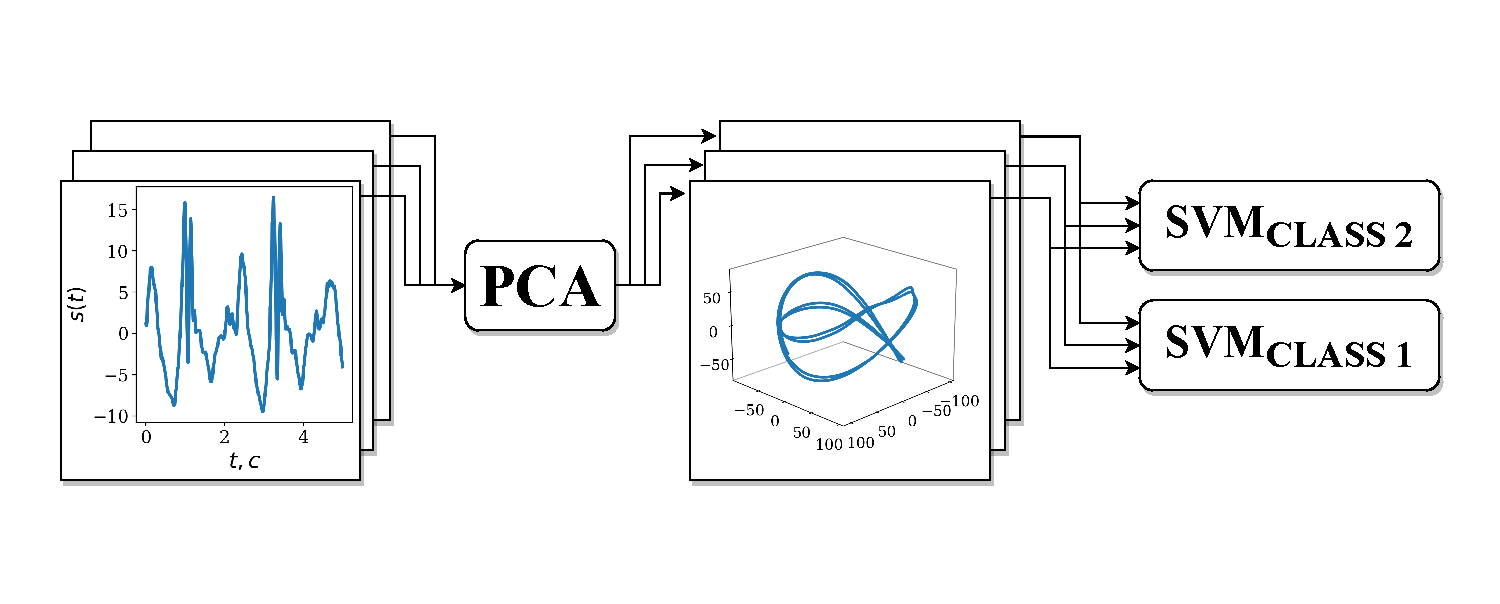
\includegraphics[scale=0.5]{./figs/PCA_SVM.pdf}
%     \caption{Схема первой версии метода классификации фазовой траектории}
%     \label{fg:alternative_pipline_v1}
% \end{figure}

% \begin{figure}[h]
%     \centering
%     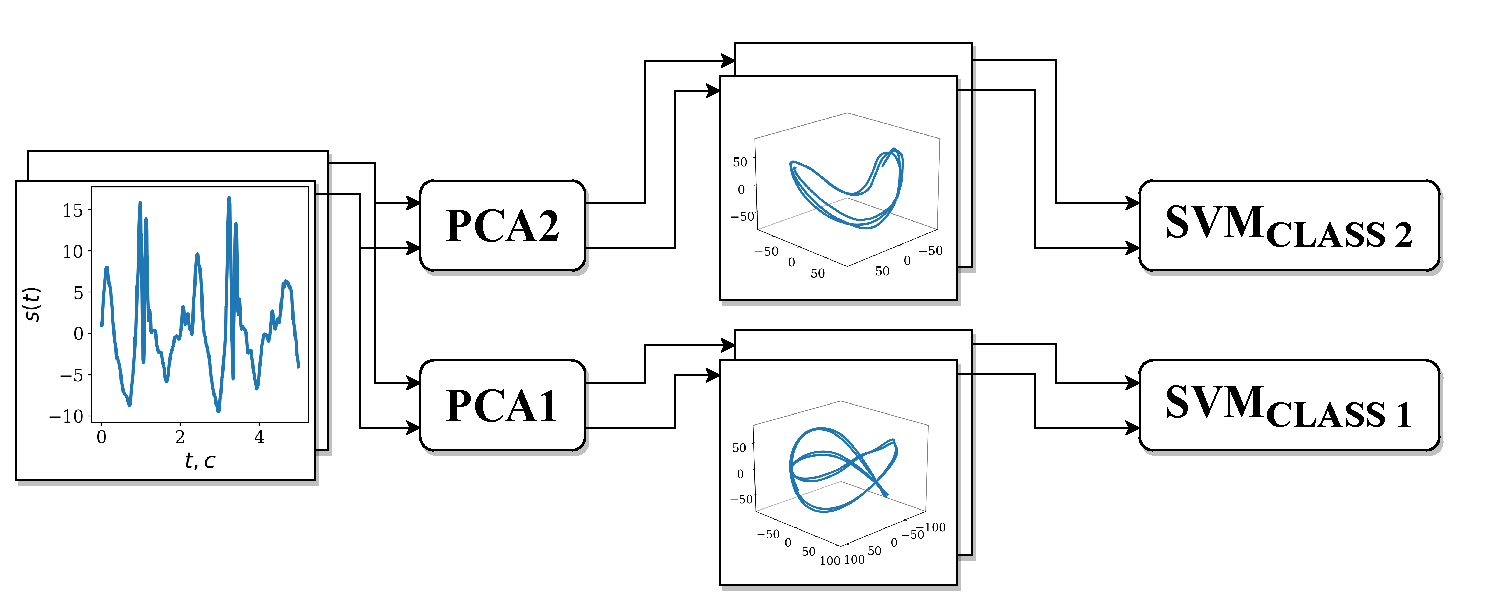
\includegraphics[scale=0.5]{./figs/TWO_UNIQUE_PCA_SVM.pdf}
%     \caption{Схема второй версии метода классификации фазовой траектории}
%     \label{fg:alternative_pipline_v2}
% \end{figure}



%%%%%%%%%%%%%%%%%%%%%%%%%%%%%%%%%%%%%%%%%%%%%%%%%%%%%%%%%%%%%%%%%%%%%%%%%%%%%
\section{Эксперимент по классификации сферическими гармониками}
Задан набор данных, измеренный датчиками акселерометра телефона.
Он собирается с частотой дискретизации 50~Гц.
Двадцать четыре участника разного пола, возраста, веса и роста выполнили три типа повторяемых физических активностей: движение по лестнице, ходьба, бег.
Более подробное описание набора данных в~\cite{Malekzadeh_2018}.
Участники имеют разные типы походки и, как следствие, разные фазовые траектории.
Поэтому были отобраны три человека со схожими показателями роста и веса.

Алгоритм классификации схож с вариантом на Рис.~\ref{fg:alternative_piplines}б. Основное отличие в аппроксимация фазовой траектории линейной комбинацией сферических гармоник как показано на Рис.~\ref{fg:alternative_piplines}в.

Размер предыстории выбирается равным $n = 150$, что советует трем секундам.
Период движений в данных не превосходит двух с половиной секунд.
Значение старшего индекса, используемого для построения модели сферических~(\ref{eq:f_sh}) гармоник, выбирается равным $N_{\text{approx}} = 10$ для размерности фазового пространства $\mathbf{H}_{x}^{p}$ равного трем, $N_{\text{approx}} = 6$ для размерности четыре и $N_{\text{approx}} = 3$ для размерности пять.
Для пространств большей размерности эксперимент не проводился из-за малого объема данных и  вычислительной неэффективности подсчета сферических гармоник для размерности пространства равной шести и более.

\begin{table}[H]
    \caption{F-score классификации на трех пользователях с одинаковым типом походки}
    \label{tbl:accuracy_table_all}
    \centering\medskip\tabcolsep=11pt\small
    \begin{tabular}{l|ccc|ccc|ccc}
        Метод
            & \multicolumn{3}{c|}{Ходьба}
            & \multicolumn{3}{c|}{Бег}
            & \multicolumn{3}{c}{Лестница}\\
        Размерность $p$
            & 3 & 4 & 5
            & 3 & 4 & 5
            & 3 & 4 & 5\\
    \headline
        {Пользователь 1}
            & $0.98$ & $0.99$ & $0.95$ % Ходьба
            & $0.97$ & $0.99$ & $0.8$ % бег
            & $0.86$ & $0.84$ & $0.92$ \\% Лестница
        {Пользователь 2}
            & $0.99$ & $0.97$ & $0.57$ % Ходьба
            & $0.98$ & $0.98$ & $0.91$ % бег
            & $0.95$ & $0.68$ & $0.86$ \\% Лестница
        {Пользователь 3}
            & $0.96$ & $0.93$ & $0.58$ % Ходьба
            & $0.89$ & $0.64$ & $0.82$ % бег
            & $0.85$ & $0.65$ & $0.86$ \\% Лестница
    \end{tabular}
\end{table}

\begin{figure}[H]
    \centering
    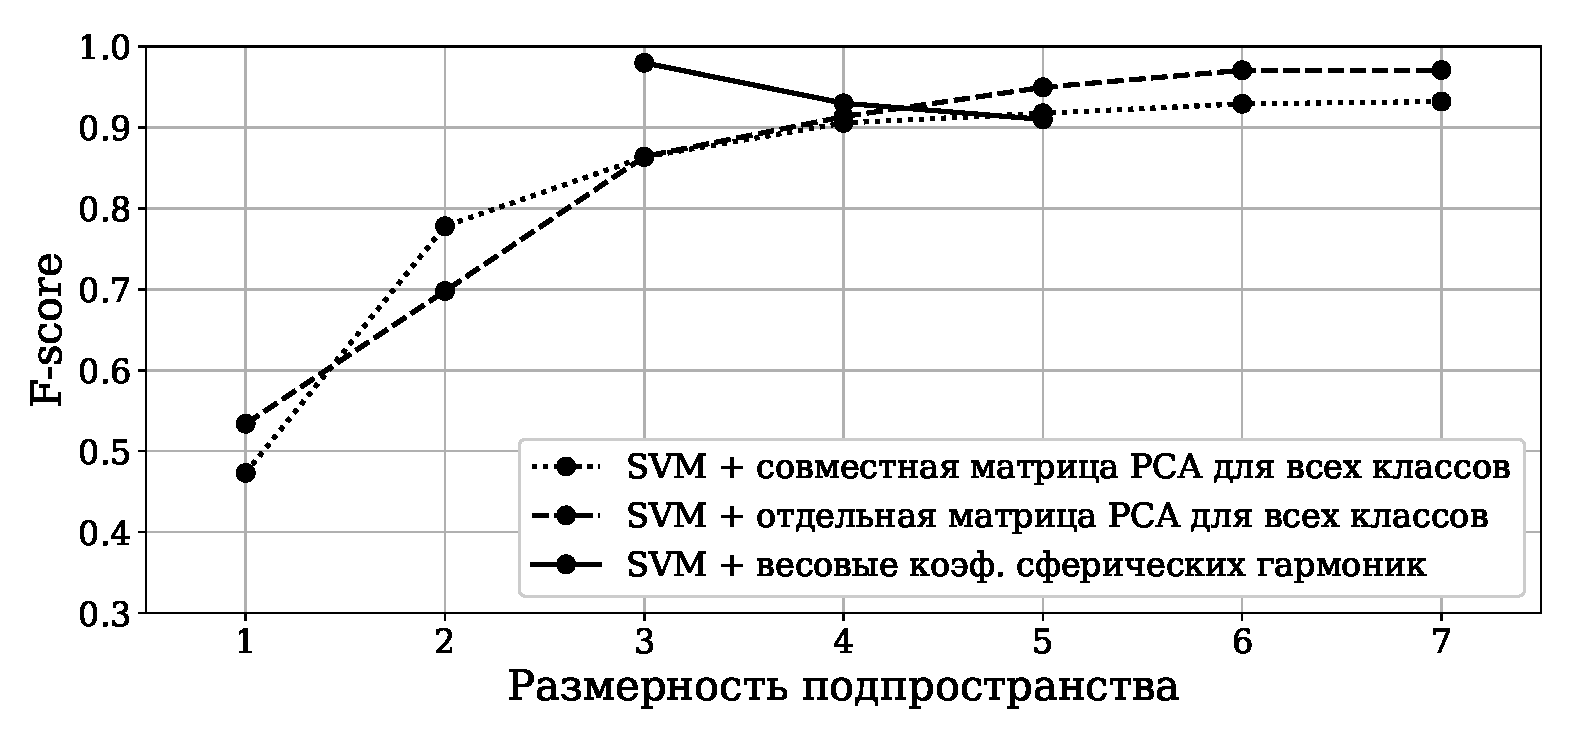
\includegraphics[scale=0.5]{./figs/result_first.eps}
    \caption{F-score на ходьбе, беге, спуску и подъему по лестнице для одного пользователя}
    \label{fg:clf_result_one}
\end{figure}

На Рис.~\ref{fg:clf_result_one} показано качество классификации F-score движении одного человека.
Видно, что для эффективной классификации достаточно трехмерных сферических гармоник.
При применении методов, обученных  на данных первого пользователя, для классификации временных рядов записанных с второго и третьего пользователей качество падает в зависимости от типа движения.
Так бег и ходьба классифицируются лучше, чем движение по лестнице.
В таблице~\ref{tbl:accuracy_table_all} представлена качество классификации для нескольких пользователей.
При этом из-за увеличения размерности пространства падает общее качество классификации. Средние значения представлены на Рис.~\ref{fg:clf_result_many} и в таблице~\ref{tbl:accuracy_table_mean}.

\begin{table}[H]
    \caption{Среднее качество классификации на трех пользователях с одинаковым типом походки}
    \label{tbl:accuracy_table_mean}
    \centering\medskip\tabcolsep=11pt\small
    \begin{tabular}{l|ccc}
        Метод & \multicolumn{3}{c}{F-score}\\
        Размерность $p$ & 3 & 4 & 5\\
    \headline
        {SVM + весовые коэф. сферических гармоник}     & $0.90$ & $0.82$ & $0.81$ \\
        {SVM + совместная матрица PCA для всех классов} & $0.79$ & $0.80$ & $0.89$ \\
        {SVM + отдельная матрица PCA для каждого класса} & $0.78$ & $0.81$ & $0.81$ \\
    \end{tabular}
\end{table}

\begin{figure}[H]
    \centering
    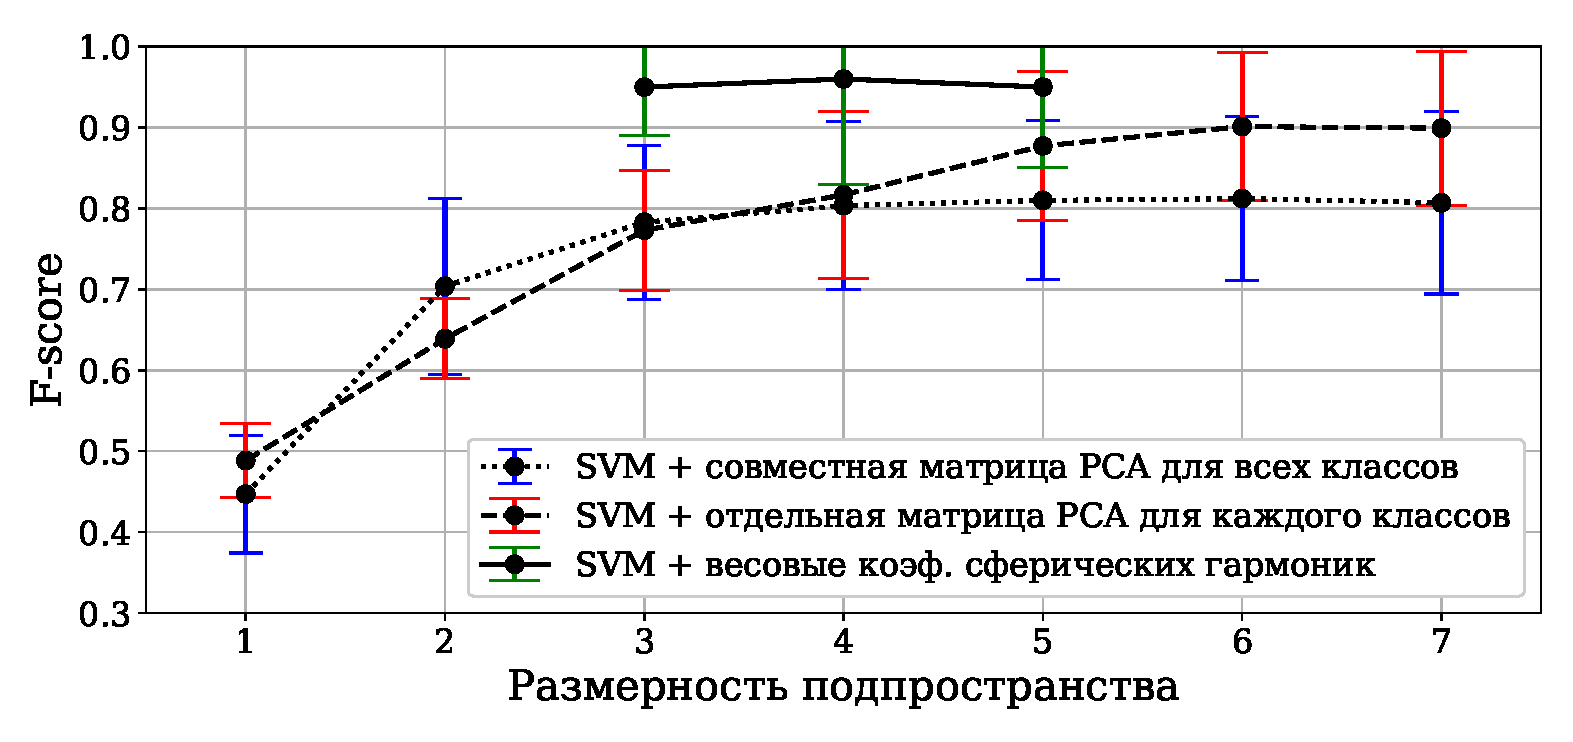
\includegraphics[scale=0.5]{./figs/result_mean.eps}
    \caption{Средний и СКО F-score на ходьбе, беге, спуску и подъему по лестнице}
    \label{fg:clf_result_many}
\end{figure}

В таблице~\ref{tbl:table_of_figures} показаны результаты работы алгоритма.
Слева фрагмент временного ряда записанного с акселерометра.
По центру полученные фазовые траектории в трехмерном пространстве.
Справа модели сферических гармоник.
Видно, что разные классы временных рядов имеют разные траектории и разные модели аппроксимации.

\begin{table}
\centering
\caption{Таблица сравнений разных классов движений}
\begin{tabular}{p{0.5cm}p{3cm}p{4cm}p{4cm}}
    & Временной ряд
    & Фазовая траектория
    & Модель
    \\
    \hline
    \rotatebox{90}{ \text{Ходьба} }
    & 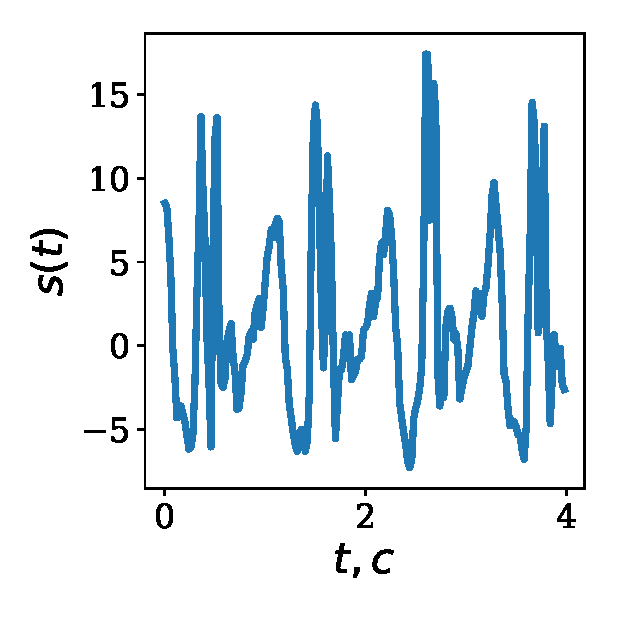
\includegraphics[scale=0.3]{figs/time_series_wlk_8.eps}
    & 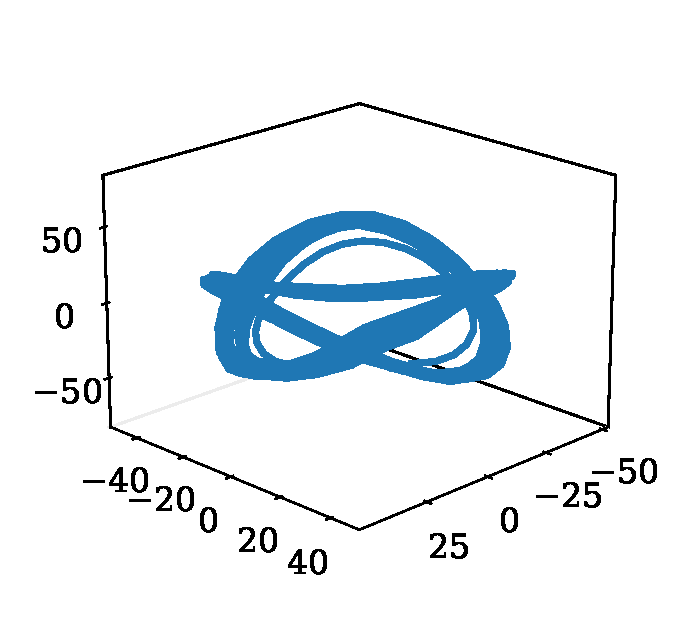
\includegraphics[scale=0.35]{figs/phase_traj_wlk_8.eps}
    & \includegraphics[scale=0.35]{figs/spharm_wlk_8.eps}
    \\ 
    \hline
    \rotatebox{90}{ \text{Бег} }
    & 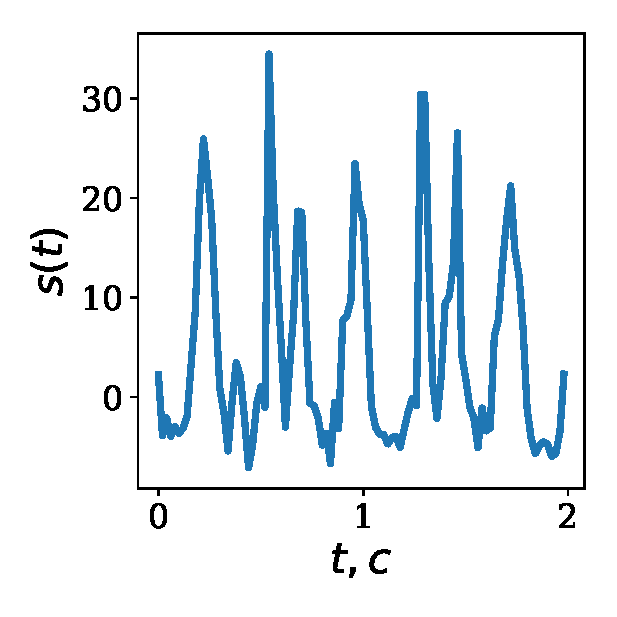
\includegraphics[scale=0.3]{figs/time_series_jog_9.eps}
    & 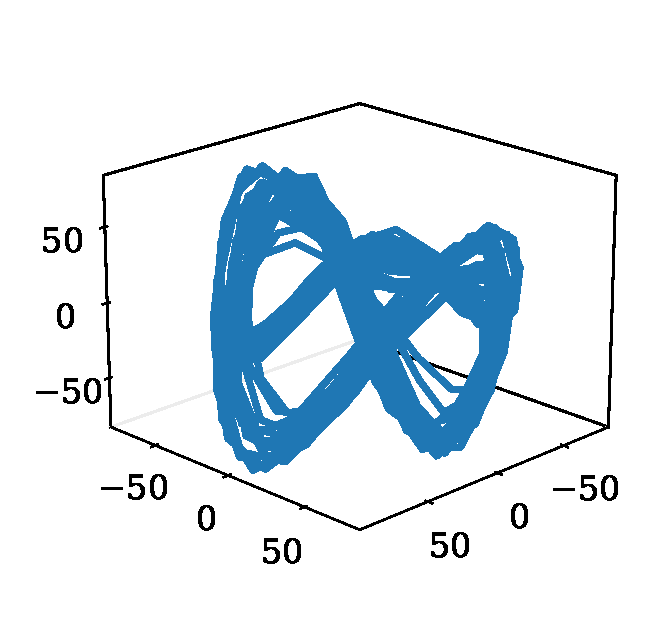
\includegraphics[scale=0.35]{figs/phase_traj_jog_9.eps}
    & \includegraphics[scale=0.35]{figs/spharm_jog_9.eps}
    \\ 
    \hline
    \rotatebox{90}{ \text{Лестница} }
    & 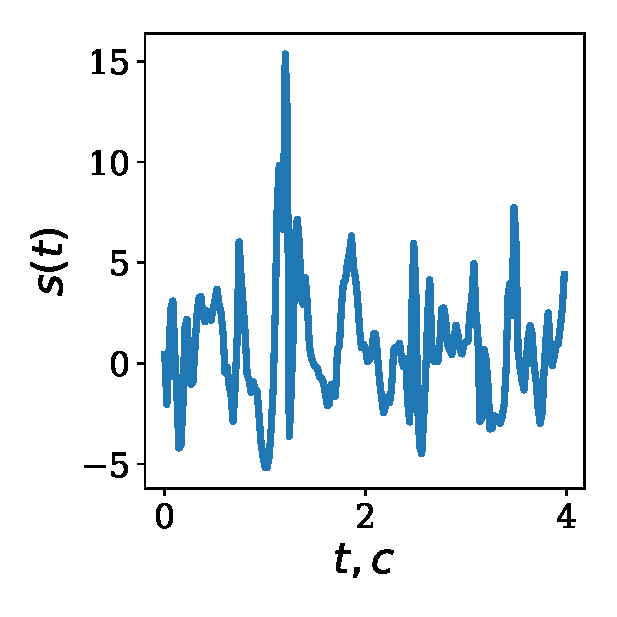
\includegraphics[scale=0.3]{./figs/time_series_ups_4.eps}
    & 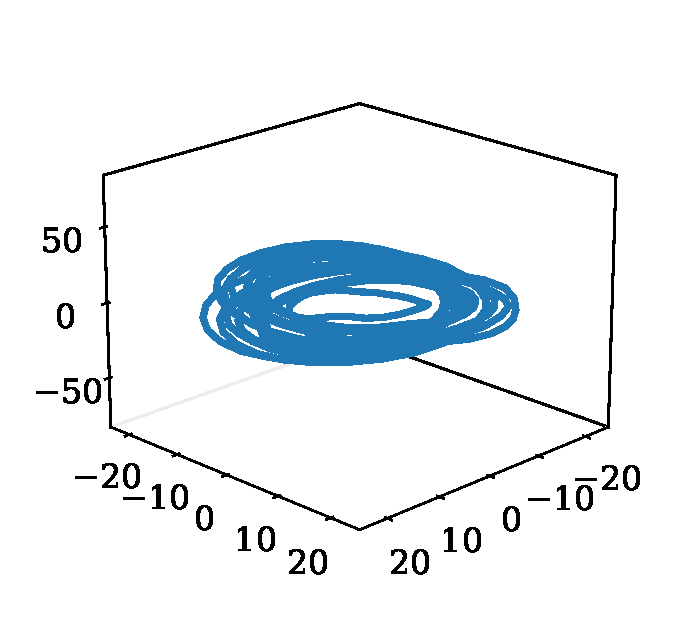
\includegraphics[scale=0.35]{./figs/phase_traj_ups_4.eps}
    & 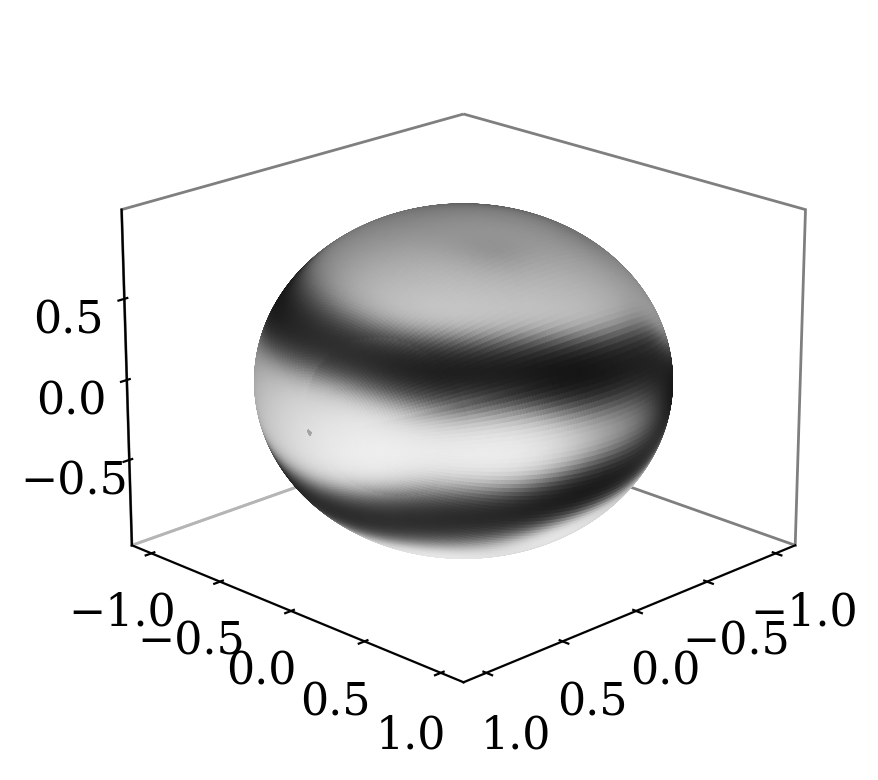
\includegraphics[scale=0.35]{./figs/spharm_ups_4.eps}
    \\ 
    \hline
\end{tabular}
\label{tbl:table_of_figures}
\end{table}

% \begin{figure}
% \centering
% \subfloat[Ходьба]
% {
%     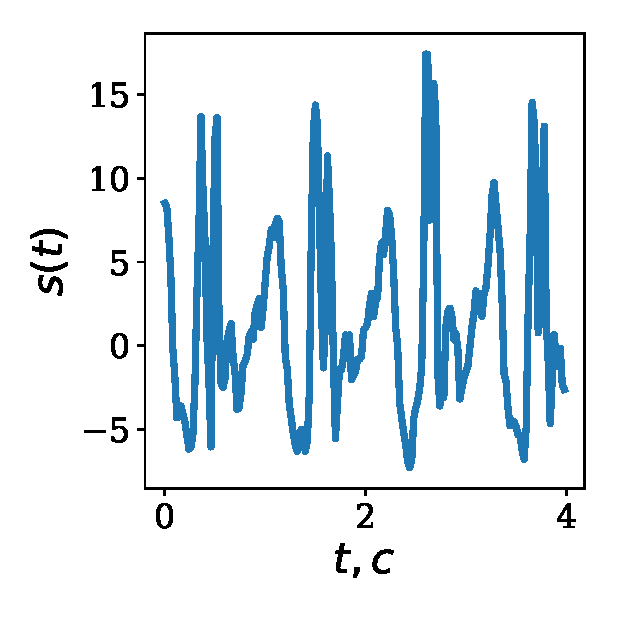
\includegraphics[width=0.15\textwidth]{figs/time_series_wlk_8.eps}
%     \quad \quad
%     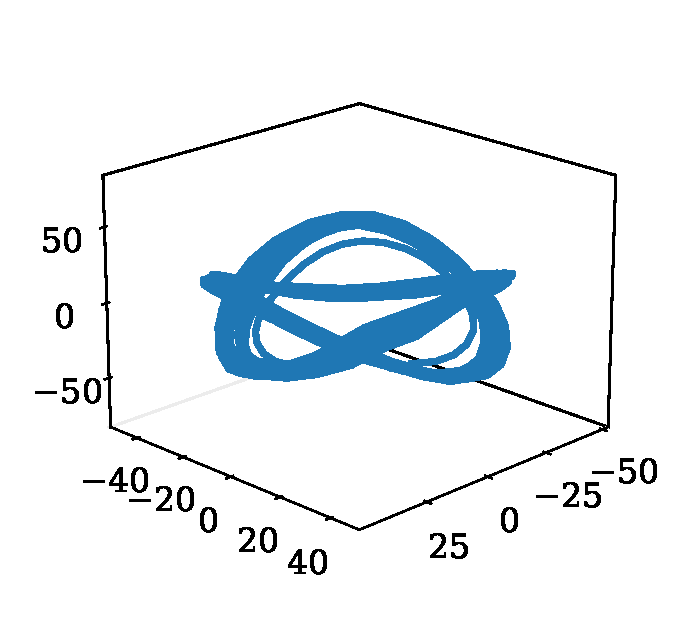
\includegraphics[width=0.2\textwidth]{figs/phase_traj_wlk_8.eps}
%     \quad \quad
%     \includegraphics[width=0.2\textwidth]{figs/spharm_wlk_8.eps}
% }\\
% \subfloat[Бег]
% {
%     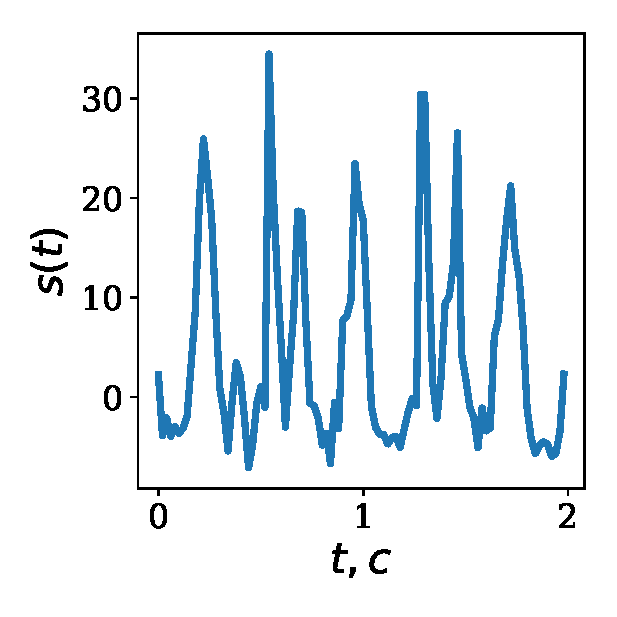
\includegraphics[width=0.15\textwidth]{figs/time_series_jog_9.eps}
%     \quad \quad
%     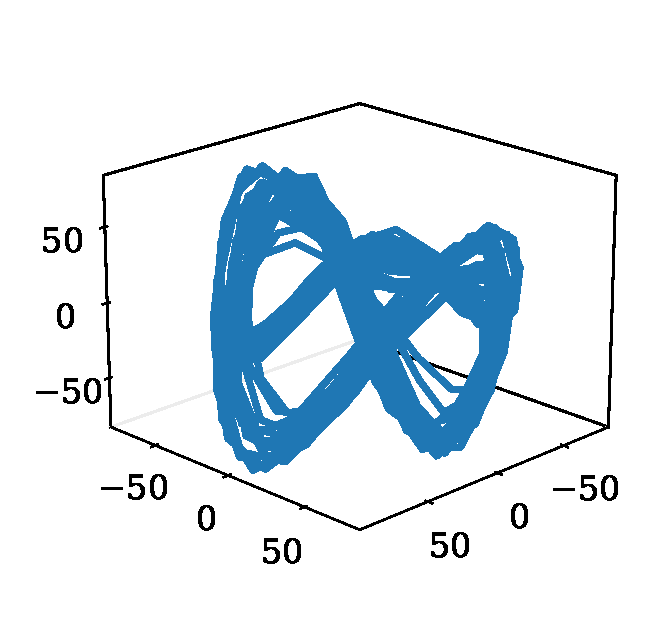
\includegraphics[width=0.2\textwidth]{figs/phase_traj_jog_9.eps}
%     \quad \quad
%     \includegraphics[width=0.2\textwidth]{figs/spharm_jog_9.eps}
% }\\
% \subfloat[Подъем по лестнице]
% {
%     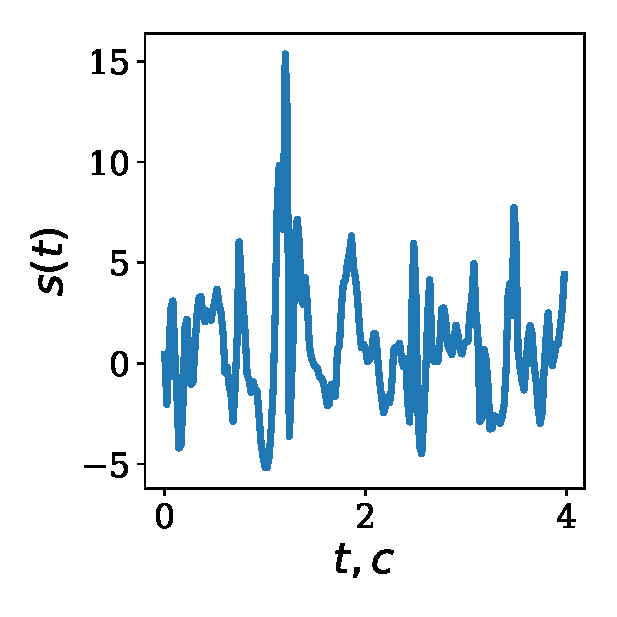
\includegraphics[width=0.15\textwidth]{figs/time_series_ups_4.eps}
%     \quad \quad
%     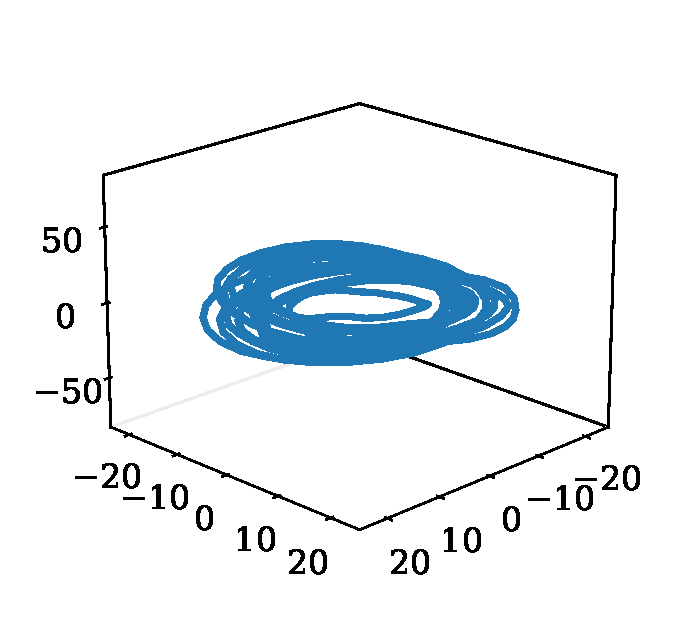
\includegraphics[width=0.2\textwidth]{figs/phase_traj_ups_4.eps}
%     \quad \quad
%     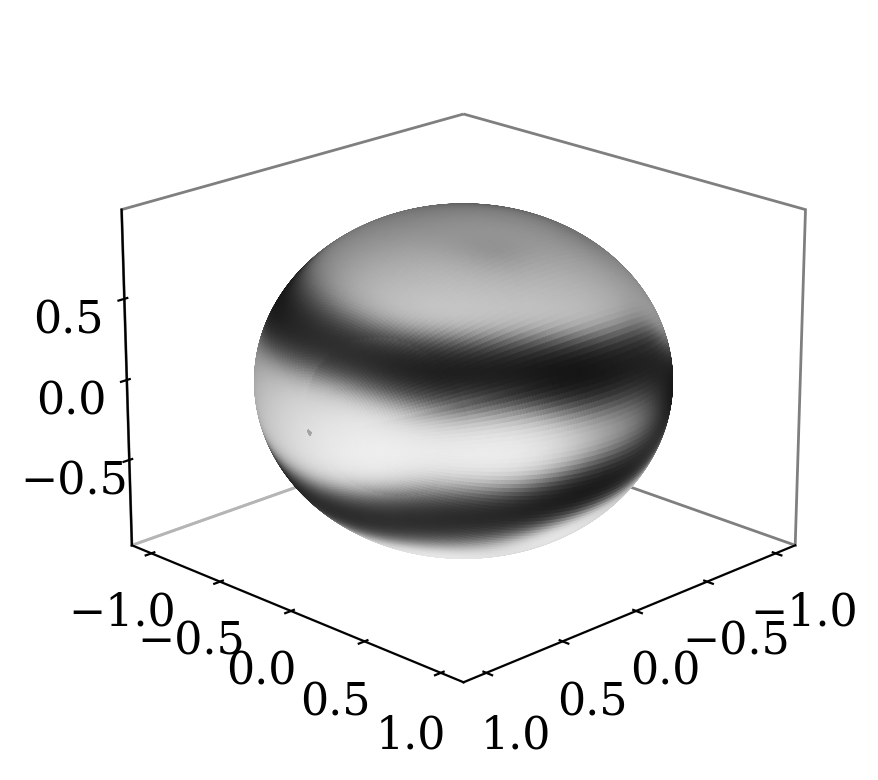
\includegraphics[width=0.2\textwidth]{figs/spharm_ups_4.eps}
% }\\
% \caption{Слева: сегмент временного ряда, по центру: фазовая траектория, справа: модель сферических гармоник.}
% \label{fg:result_experiment}
% \end{figure}

% \begin{figure}[h]
%     \centering
%     \includegraphics[scale=0.3]{figs/3_pic_wlk_8.eps}
%     \caption{F-score на ходьбе, беге, спуску и подъему по лестнице для одного человека}
%     \label{fg:clf_result_one}
% \end{figure}

% \begin{figure}[h]
%     \centering
%     \includegraphics[scale=0.3]{figs/3_pic_jog_9.eps}
%     \caption{F-score на ходьбе, беге, спуску и подъему по лестнице для одного человека}
%     \label{fg:clf_result_one}
% \end{figure}

% \begin{figure}[h]
%     \centering
%     \includegraphics[scale=0.3]{figs/3_pic_ups_4.eps}
%     \caption{F-score на ходьбе, беге, спуску и подъему по лестнице для одного человека}
%     \label{fg:clf_result_one}
% \end{figure}


%%%%%%%%%%%%%%%%%%%%%%%%%%%%%%%%%%%%%%%%%%%%%%%%%%%%%%%%%%%%%%%%%%%%%%%%%%%%%%%%%%%%%%%%%%
\section{Заключение}

В работе решалась задача классификации квазипериодических временных рядов, а также задача построения модели фазовой траектории.
Для снижения размерности траекторного подпространства к фазовой траектории применялся метод главных компонент.
Фазовая траектория, представленная в сферических координатах, аппроксимировалась линейной комбинацией сферических гармоник.

Эксперимент проводился на трех временных рядах: показатели акселерометра во время ходьбы, бега и спуска по с лестницы для трех пользователей с близкими показателями роста и веса.
Качество классификации высокое при оценке на пользователе, на котором обучались модели.
Модели фазовых траекторий на поверхности сферы показали, что такая аппроксимация сохраняет геометрическую структуру последовательности точек, а также содержит информацию о математическом ожидании и дисперсии фазовой траекторию.
Это хорошо видно в таблице~\ref{tbl:table_of_figures} на рисунках справа.
Темно серая область на поверхности сферы представляет собой дисперсию фазовой траектории, более черная --- математическое ожидание.
Свойства модели аппроксимации будут отдельно исследовать в будущих работах.
Количество моделей остается небольшим по сравнению с нейронными сетями или ближайшими соседями.
Каждый этап классификации имеет явную интерпретацию.
\newpage
\bibliography{lib}

\end{document}
